\documentclass{article}


\usepackage{amsmath} % math stuff
\usepackage{amssymb} % math stuff
\usepackage{array} % equations and stuff
\usepackage{bm} % bold math
%\usepackage{caption} % suppressed table numbering; incompatible with revtex, and longtable, I think
\usepackage{comment} % comment environment
%\usepackage{enumitem} % customization of enumeration, itemize, and description
\usepackage[T1]{fontenc} % font encoding for special characters, must also use scalable font package
\usepackage[margin=0.8in]{geometry} % paper sizes and margins (but be careful not to mess up pre-defined pages)
\usepackage{graphicx} % for graphics
%\usepackage{helvet} % default font is the helvetica postscript font
\usepackage{lipsum} % lorem ipsum filler text
\usepackage{lmodern} % scalable font?
\usepackage{longtable} % multi-page tables
\usepackage{mathrsfs} % math script font
\usepackage{mhchem} % easier chemical formula
\usepackage{microtype} % allows disabling of ligatures
%\usepackage{newcent} % new century schoolbook font
\usepackage{nicefrac}
\usepackage{parskip} % removes paragraph indentation, and adjusts paragraph skip, as well as list items
%\usepackage{setspace} % adjust text spacing and indents
\usepackage{siunitx} % decimal alignment
\usepackage{subfigure} % divided figures
%\usepackage{tabu} % extra table options
\usepackage{textcomp} % symbols
\usepackage{threeparttablex} % better footnotes with longtable
\usepackage{titling} % title placement
\usepackage{ulem} % strikethrough text
%\usepackage{url} % superceded by hyperref
\usepackage{verbatim} % verbatim environment
\usepackage{xcolor} % colors and color boxes
\usepackage{xspace} % commands that don't eat up white space
\usepackage{hyperref} % links and page setup; should always come last

\hypersetup{
	bookmarks=true,
	colorlinks=true,
	citecolor=blue,
	linkcolor=blue,
	urlcolor=blue,
	pdfstartview={XYZ null null 1.0} % default open view is 100%
}

\DisableLigatures[f]{encoding = *, family = * } % disable ff, fi, fl ligatures, without f option, it also disables -- = endash
\renewcommand{\arraystretch}{1} % extra vertical space in tables

\begin{document}

\pagestyle{empty} % don't number pages

% custom title
\begin{center}
{\LARGE Classic Riddler}

\vspace{0.15in}

{\Large 5 June 2020}
\end{center}


\section*{Riddle:}

The astronomers on planet Xiddler have made several remarkable discoveries.
After inventing the telescope, they quickly discovered a new planet in their solar system!

Xiddler is very much like Earth.
The planet orbits its star in a nearly circular path, with an average distance of 150 million kilometers, a period of one Earth year and a day that lasts 24 hours.
But unlike Earth, there weren't any other known planets in the solar system\dots until now.

Moments after the Xiddlerian sun set below the horizon, three astronomers happened to focus their telescopes at the zenith of the evening sky, all seeing the same new planet.
In their excitement, the astronomers race to Xiddler's Grand Minister to deliver the momentous news.

The first astronomer says that, by her calculations, the newly discovered planet orbits their sun with a radius of 50 million kilometers.
The second astronomer says that, by her calculations, the planet in fact orbits their sun with a radius of 300 million kilometers.
The third astronomer disagrees with the other two---by her calculations, the planet has a very similar orbit to Xiddler, with a radius of 150 million kilometers.

Which astronomer should the Grand Minister believe?

\section*{Solution:}

I have created a diagram that illustrates the riddle below.
The orbits of the three planets are to scale, even if the sun and planet are too large.

\begin{center}
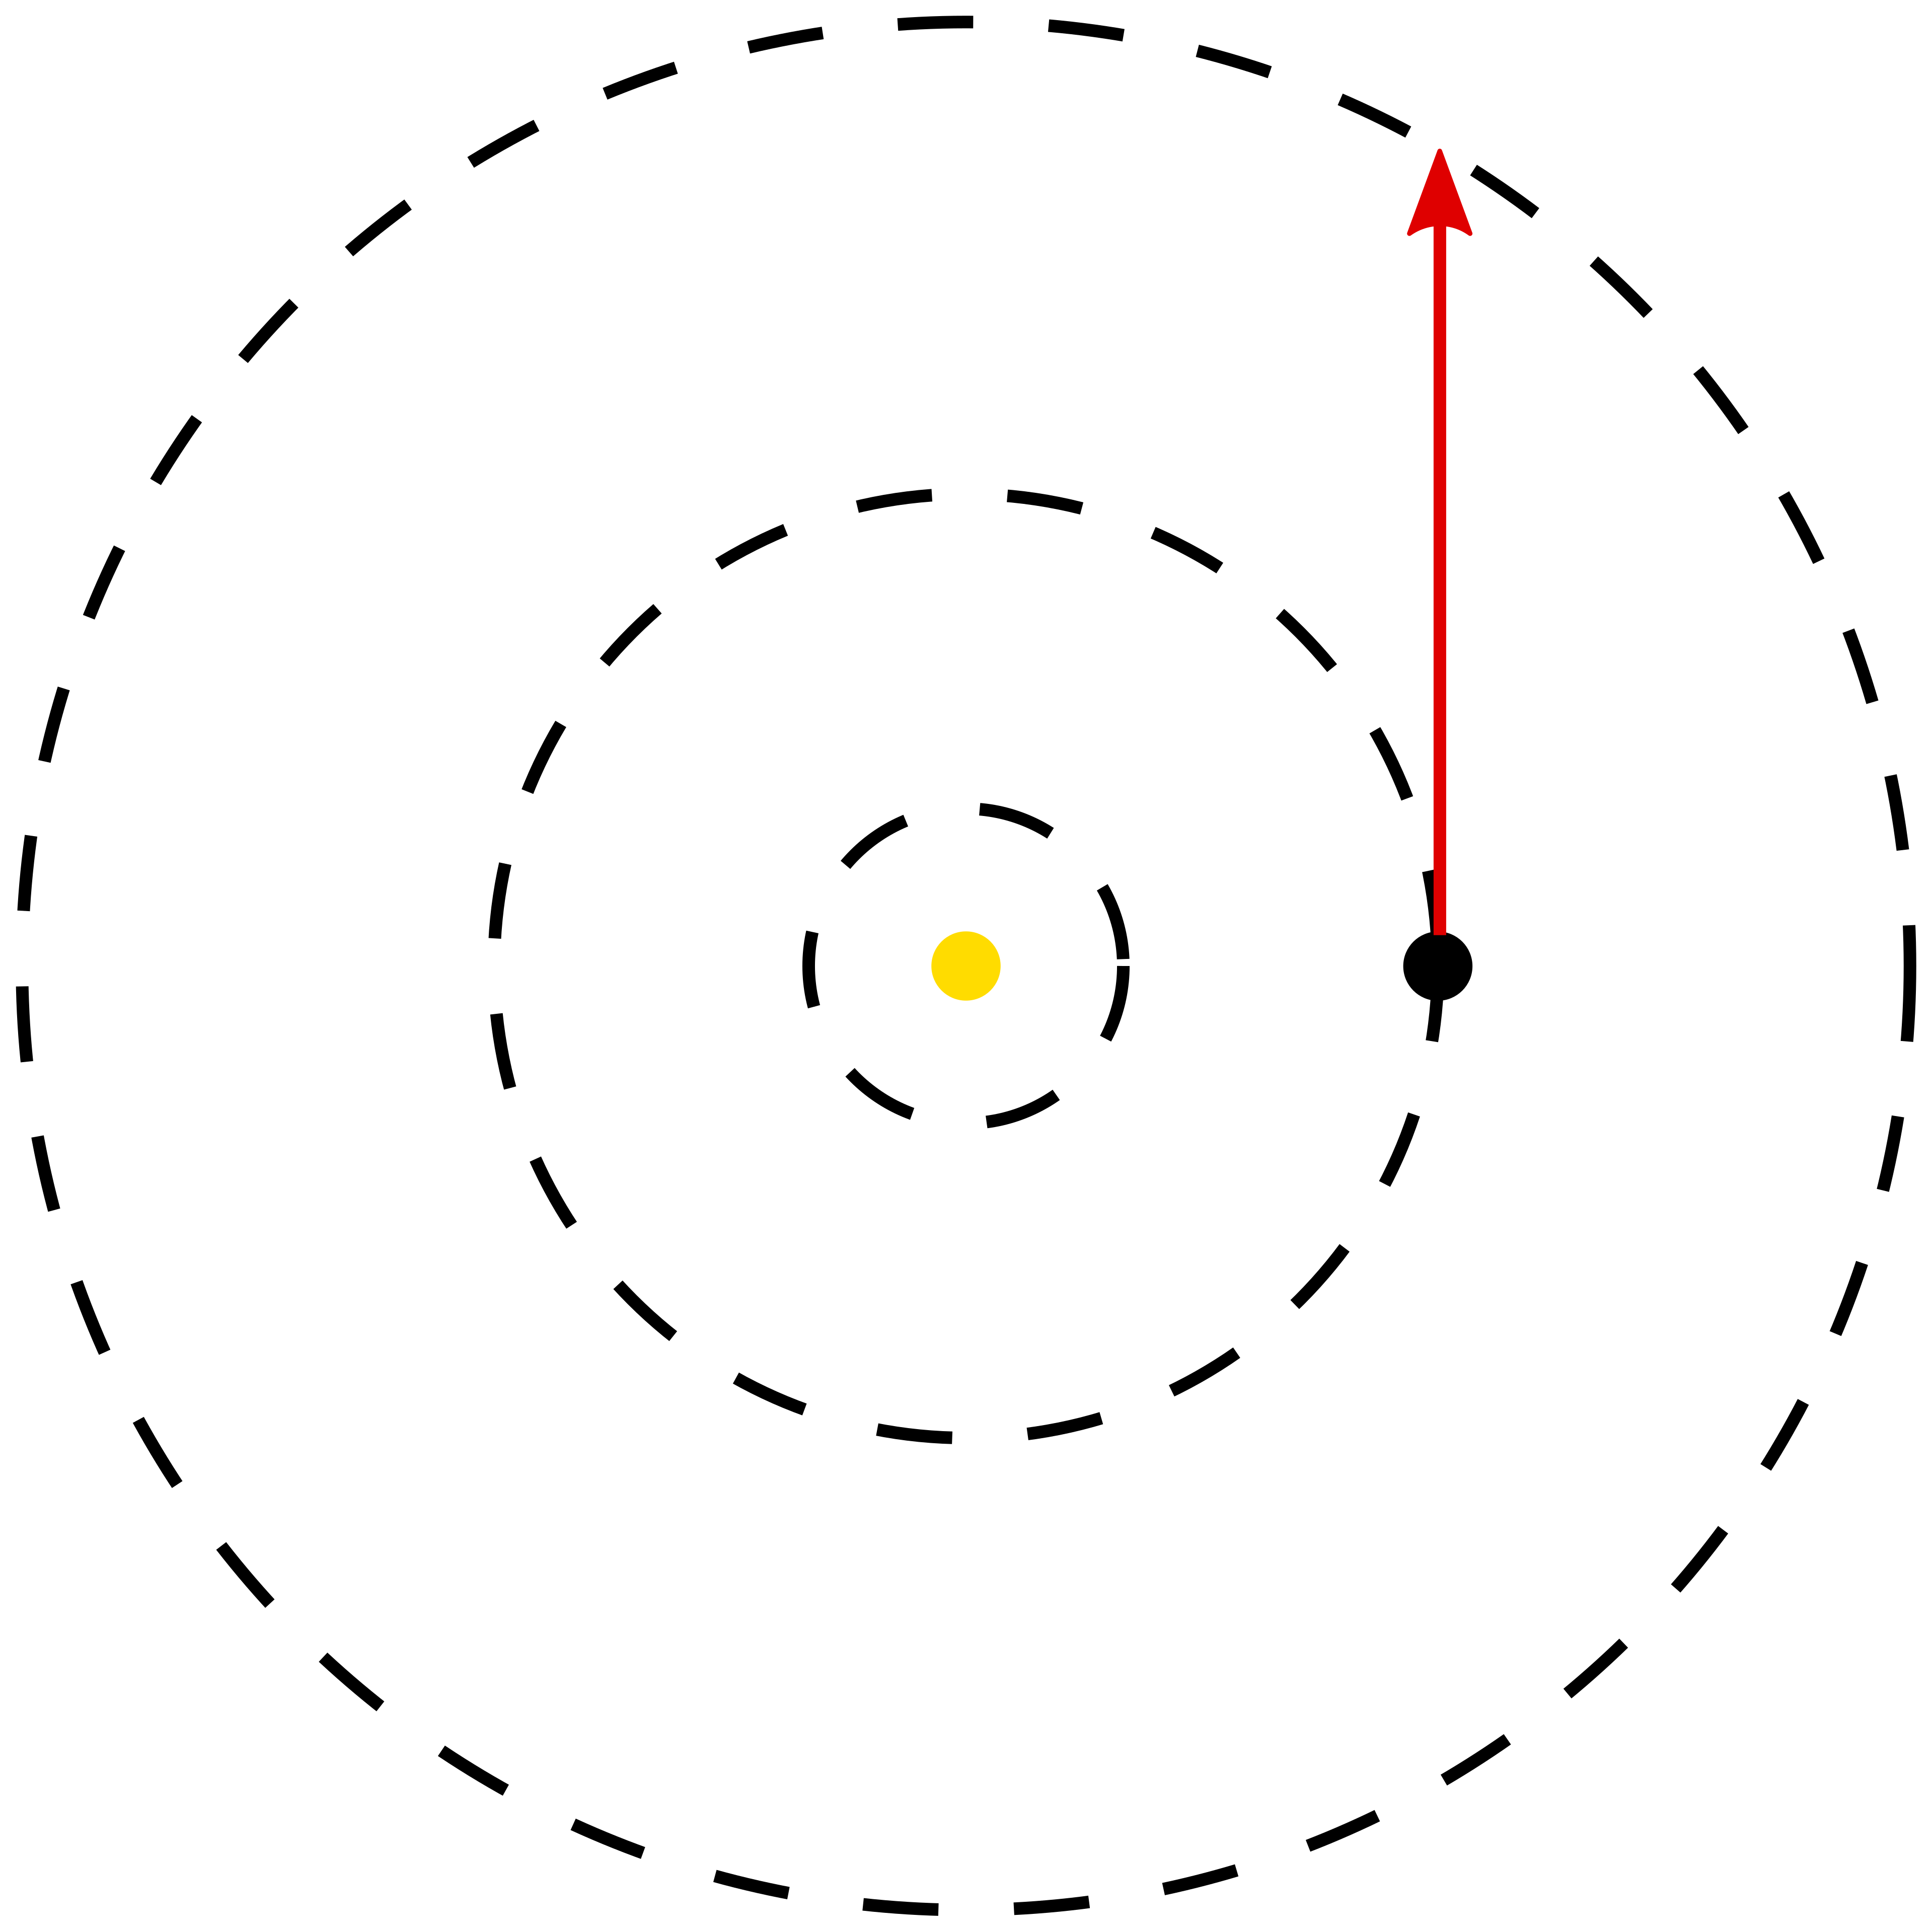
\includegraphics[width=3.5in]{solar_system.png}
\end{center}

Just at sunset, the astronomers are located at an edge that perpendicular to the distance from the sun, and if they look to the sky's zenith, they are looking in the direction of the red arrow.
It is clear that only the largest orbit is within sight of the arrow, so the radius which is most likely to be correct, and the riddle's solution, is
\fcolorbox{red}{white}{\bf 300 million kilometers}\,.
From the given information, there is no reason the answer must specifically be 300, but that astronomer is the only one with the correct logic: that the orbital radius must be larger than Xiddler's orbital radius.

\end{document}